% ------------------------------------------------------------
% Page 106
% ------------------------------------------------------------

\begin{wrapfigure}{l}{0.42\textwidth}
    \centering
    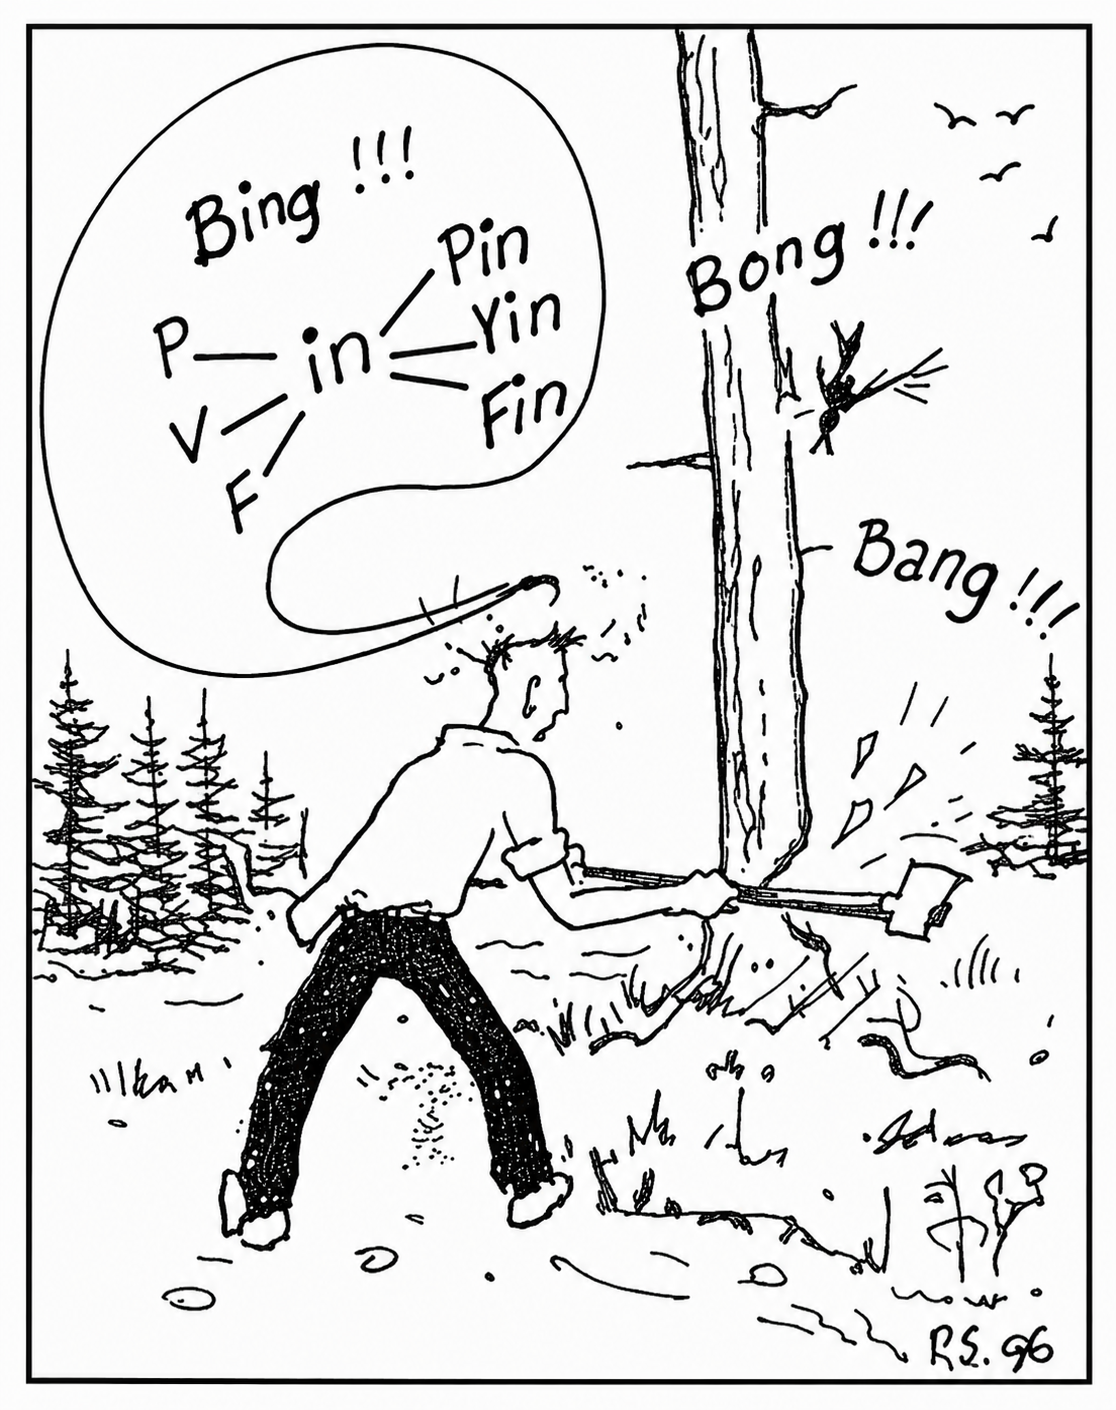
\includegraphics[width=\linewidth]{imgs/113}
\end{wrapfigure}

Le « voyage de bois » non scié, fourni par
M. le Maire ne résista pas longtemps aux
besoins confondus du poêle de l’école et
de notre cuisinière.
Par nécessité je devins alors instituteur
bûcheron et, dès la fin novembre je
passais le plus clair de mes jeudis et
dimanches dans la forêt domaniale qui
s’étendait jusqu’à la Serreyrède.
Moyennant une redevance de 6 F versés
au garde-forestier de Valbelle, je pouvais
couper parmi les arbres morts,
complètement ébranchés, tout ce qui était
à ma convenance. J’avais une bonne
hache et assez d’expérience pour orienter
la chute des troncs en tous points
semblables à de longs poteaux
télégraphiques.

Tout au long de la route forestière, j’étalais donc l’équivalent de deux gros « voyage »
que le père de Martin, fort gentiment et gratuitement : me ramena jusqu’à l’école.
Commença alors le long et combien pénible travail de sciage. La « tronçonneuse »
d’alors, donc la scie à mains, même bien affûtée, graissée, ne fonctionnait « qu’à
l’huile de coude ».

Fendre les rondins obtenus en quatre bûches n’était alors qu’un jeu. Marin, qui avait
la responsabilité du poêle et du bûcher, s’activait pour dresser et équilibrer les piles
de bois devant la grande porte, selon les conseils de M. l’Inspecteur, pour éviter les
courants d’air.

\textbf{L’environnement}

L’école ne disposait pas de WC. Il n’en restait pas moins que, comme tous les
mortels, il fallait satisfaire à certains besoins « biologiques ». Au cours de
promenades matinales j’acquis une connaissance précise de l’environnement et des
possibilités d’en tirer avantage.

La cuisinière allumée, la tasse de café avalée, par tous les temps, plus ou moins
chaudement vêtu, je partais.... promener. La chance voulut que, dès mes premières
sorties, des grives (draines), des merles s’envolent de deux sorbiers au bord d’un ru.
Je ne fus pas long à comprendre. Dès lors mon fusil, ramené des Grottes lors de ma
première visite, devint le compagnon idéal. Mes chasses, bien sûr, n’intéressent
personne mais je les cite seulement pour dire que de novembre à fin mars il y eut
toujours des grives à la maison. Les jours de grive, de brouillard ou de neige
poudreuse les litornes s’abattaient par centaines sur les genévriers découverts un peu
plus haut. Une salve meurtrière, je ramassais les victimes et rentrais en courant,
pressé de glisser mes pieds sur la plaque chaude du four de la cuisinière. Ma femme
s’occupait du reste. Elle évoqua souvent les souvenirs gourmands de ses préparations
en salmis, à la tartine.
